\documentclass[10pt]{standalone}
\usepackage{commands}

\begin{document}
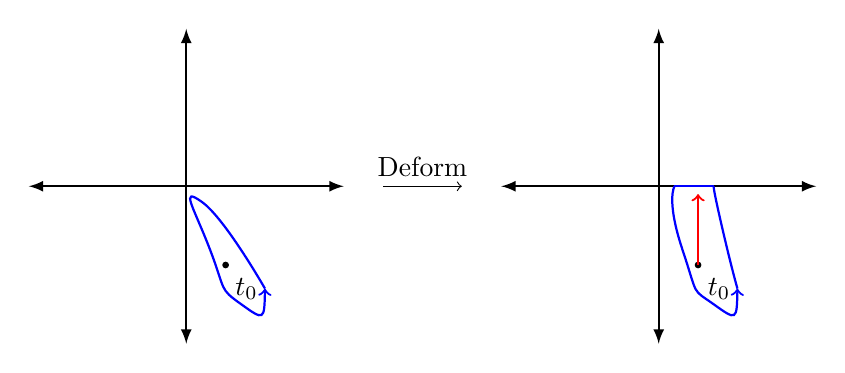
\begin{tikzpicture}
    \draw[thick, latex-latex] (-2, 0) -- (2, 0);
    \draw[thick, latex-latex] (0, -2) -- (0, 2);
    \draw[fill=black] (0.5, -1) circle (1pt);
    \node[right] at (0.5, -1.3) {$t_0$};
    \draw[blue, <-, thick] plot [smooth, tension=1.5] coordinates {(1,-1.3) (0.7,-1.5) (0.3, -0.8) (0.2, -0.2) (1, -1.3)};

    \draw[->] (2.5, 0) -- (3.5, 0);
    \node[above] at (3, 0) {Deform};

    \draw[thick, latex-latex] (4, 0) -- (8, 0);
    \draw[thick, latex-latex] (6, -2) -- (6, 2);
    \draw[fill=black] (6.5, -1) circle (1pt);
    \node[right] at (6.5, -1.3) {$t_0$};
    \draw[blue, <-, thick] plot [smooth, tension=1.5] coordinates {(7,-1.3) (6.7,-1.5) (6.3, -0.8) (6.2, 0)};
    \draw[blue, thick] plot [smooth, tension=1.5] coordinates {(7, -1.3) (6.8, -0.5) (6.7, 0)};
    \draw[blue, thick] (6.7, 0) -- (6.2, 0);
    \draw[red, thick, ->] (6.5, -1) -- (6.5, -0.1);
\end{tikzpicture}
\end{document}